\documentclass[11pt]{article}

\usepackage{graphicx}
\graphicspath{{./images/}}

\setlength{\textwidth}{430pt}\setlength{\oddsidemargin}{11pt}

\title{MATH 327 - Build Your Own Assesment}
\author{Names: Aiden Taylor (30092686), Noah Pinel (30159409)}
\date{Assesment due: Dec. 22nd, 2022}

\begin{document}

\maketitle
%\begin{center}
%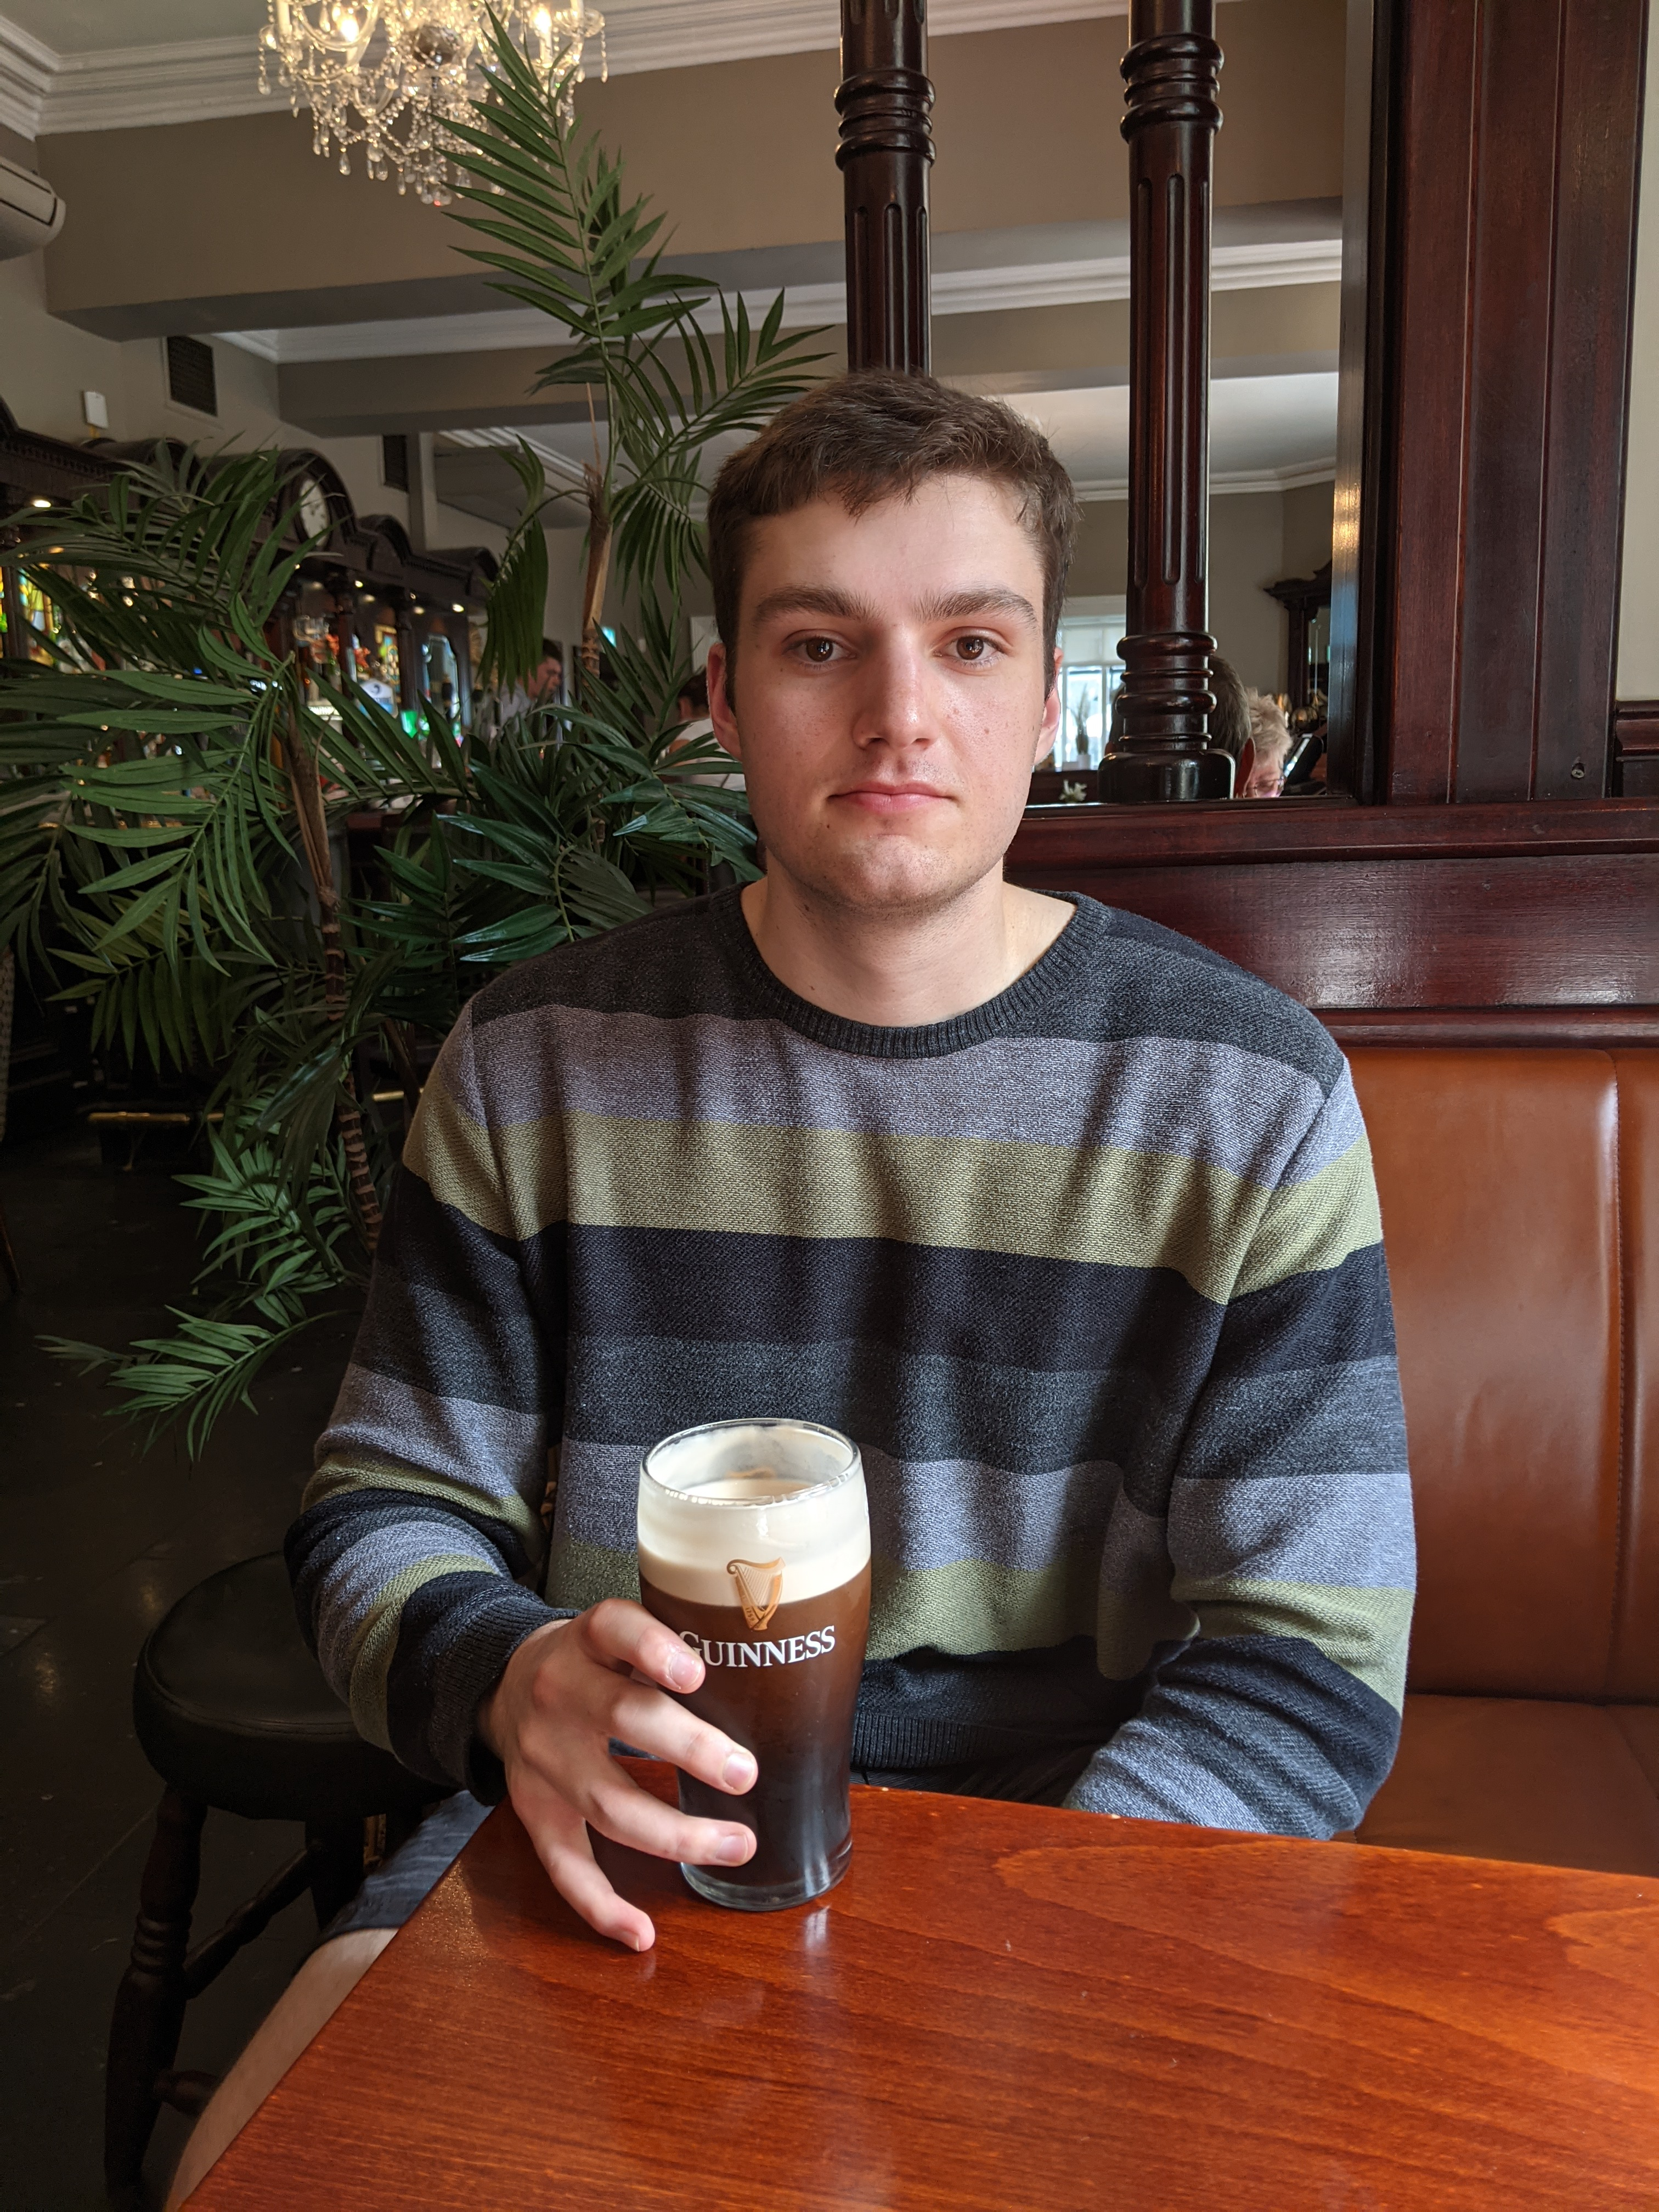
\includegraphics[scale=0.0536]{aiden}
%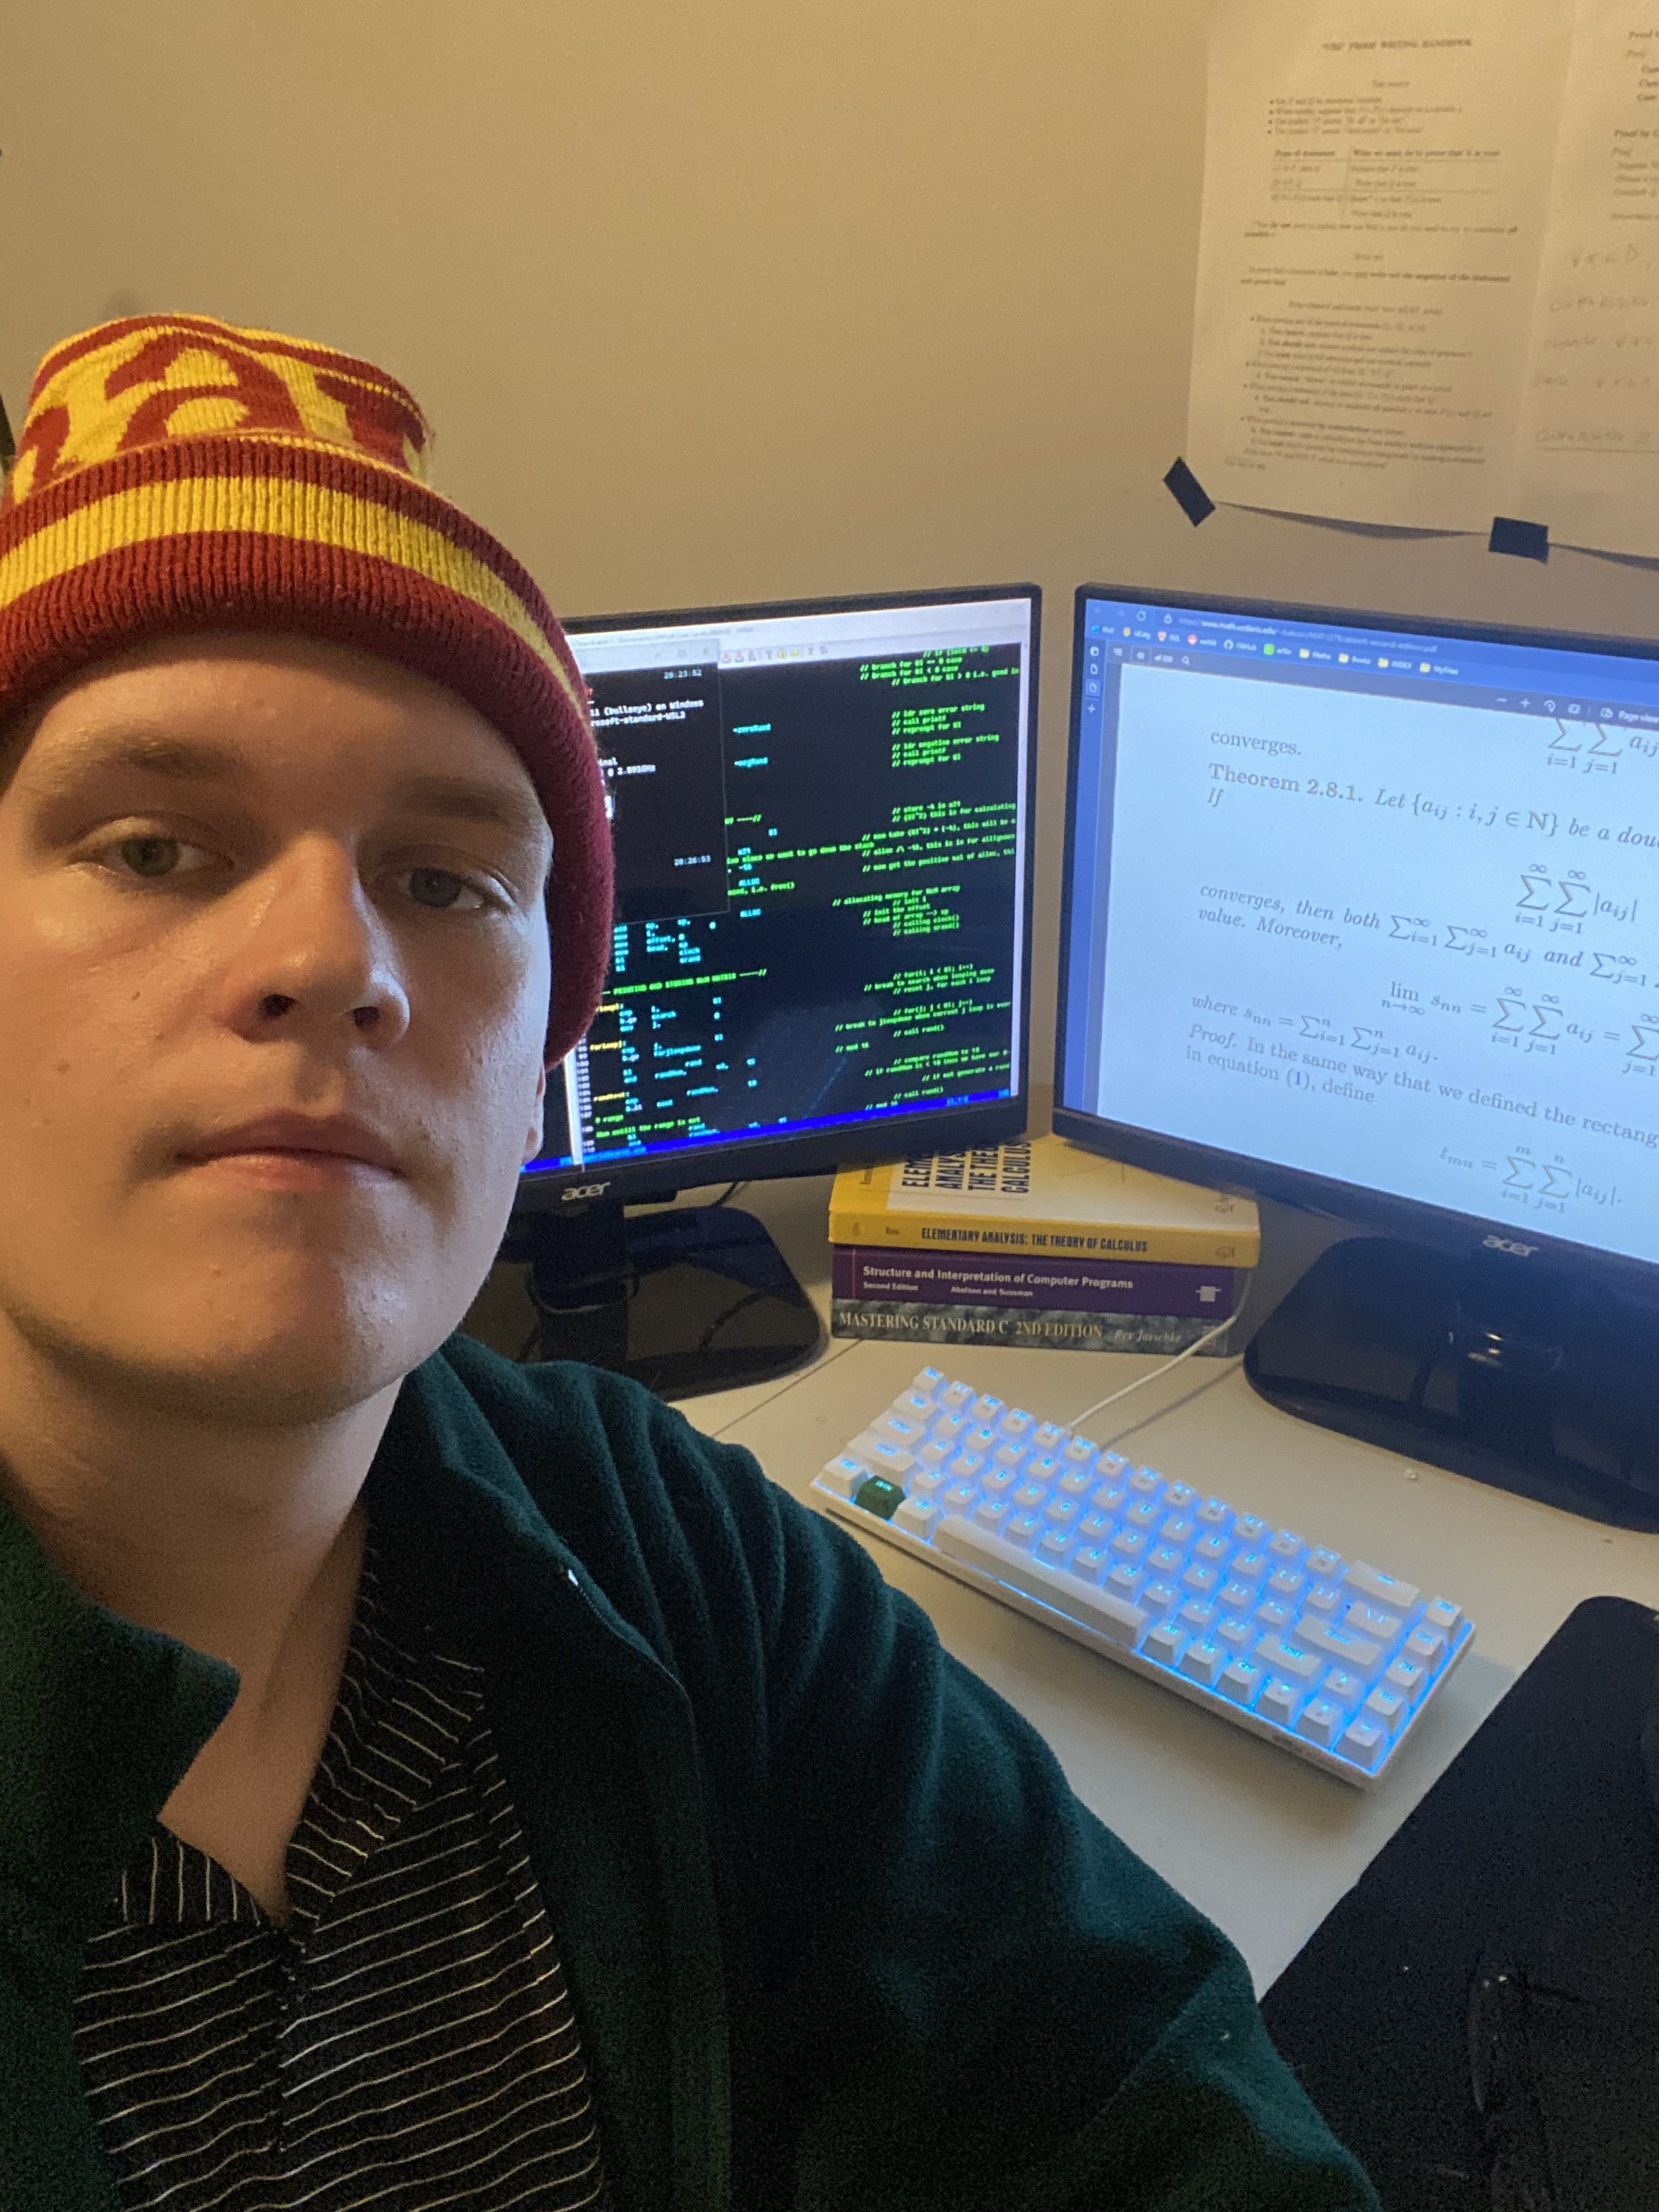
\includegraphics[scale=0.07]{noah}
%\end{center}
\newpage
\section*{Proposal}
For our assessment, we would like to make a collection of programs that are related to topics we learn in the field of Number Theory.
Our assessment idea stems from the fact that Noah and I are both Computer Science majors, and we were already interested in making programs related to topics in this class, so we thought why not group up and do this together.
Now related to our assessment, when we say a collection of programs we are intentionally being vague as we are still in the early planning phase.
Also, if interested, we have made a GitHub repository, and if needed, any instructors can be added to see the progress throughout the semester.
\section*{Program Ideas}
Below are some ideas of programs that we plan to implement for this assessment:
\begin{itemize}
\item Program that plots the first however many perfect numbers on a cartesian plane.
\item Program that visualizes congruence classes.
\item Program that either visualizes or simply calculates primes using a prime sieve.
\item Program that calculates runtimes of different primality test algorithms, and plots these runtimes.
\item Linear Diophantine Equation, GCD/LCM, and Divisor-sum function calculators.
\item etc...
\end{itemize}
These are just rough ideas for programs which will be up for change or revision as the semester continues.
Ideally, we would like to implement as many as possible, but we are aiming for around 5-10 individual programs.
\section*{Assessment Overview}
The general structure of our assessment will be:
\begin{itemize}
\item Implementation of programs related to topics in Number Theory.
\item Write-up explaining the mathematics of each program.
\item Recorded demonstration of each program supplemented by the write-up.
\end{itemize}
This structure is also up for revision, and any feedback is greatly appreciated. Thank you.
\end{document}
